\documentclass[11pt,letterpaper]{article}
\usepackage[lmargin=1in,rmargin=1in,tmargin=1in,bmargin=1in]{geometry}
\usepackage{../style/homework}
\usepackage{../style/commands}
\setbool{quotetype}{true} % True: Side; False: Under
\setbool{hideans}{false} % Student: True; Instructor: False

% -------------------
% Content
% -------------------
\begin{document}

\homework{4: Due 10/06}{I am serious. And don't call me Shirley.}{Dr. Rumack, Airplane}


% Problem 1
\problem{10} Determine if the relations $f(x)$ and $g(x)$ shown below are functions. Explain why or why not. 
	\[
	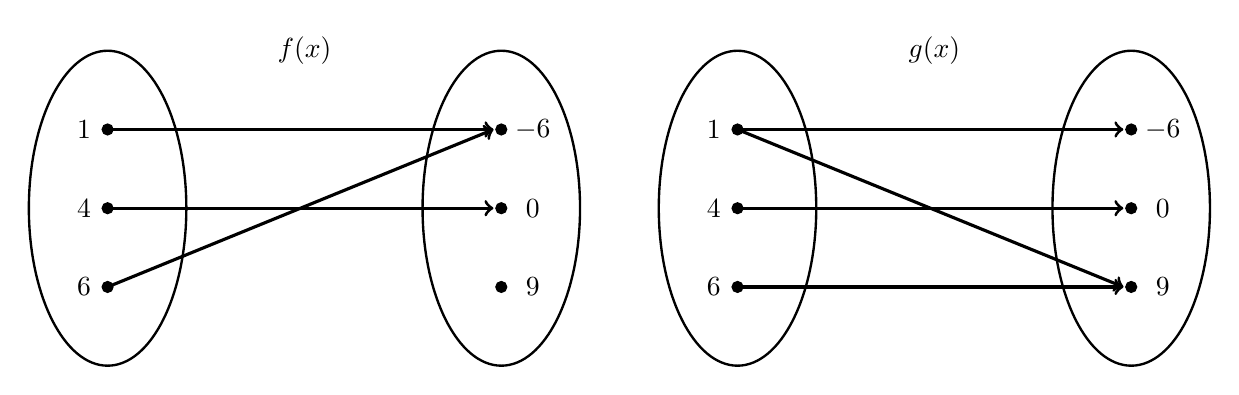
\begin{tikzpicture}
	\node at (2.5,2) {$f(x)$};
	% Ellipses
	\draw[line width=0.03cm] (0,0) circle (1 and 2);
	\draw[line width=0.03cm] (5,0) circle (1 and 2);
	
	% Nodes
	\draw[fill=black] (0,1) circle (0.07);
	\draw[fill=black] (0,0) circle (0.07);
	\draw[fill=black] (0,-1) circle (0.07);
	
	\draw[fill=black] (5,1) circle (0.07);
	\draw[fill=black] (5,0) circle (0.07);
	\draw[fill=black] (5,-1) circle (0.07);
	
	% Arrow
	\draw[line width=0.04cm,->] (0,1) -- (4.9,1);
	\draw[line width=0.04cm,->] (0,0) -- (4.9,0);
	\draw[line width=0.04cm,->] (0,-1) -- (4.9,1);
	
	% Labels
	\node at (-0.3,1) {$1$};
	\node at (-0.3,0) {$4$};
	\node at (-0.3,-1) {$6$};
	
	\node at (5.4,1) {$-6$};
	\node at (5.4,0) {$0$};
	\node at (5.4,-1) {$9$};
	
	\tikzset{shift={(8,0)}}
	%
	\node at (2.5,2) {$g(x)$};
	% Ellipses
	\draw[line width=0.03cm] (0,0) circle (1 and 2);
	\draw[line width=0.03cm] (5,0) circle (1 and 2);
	
	% Nodes
	\draw[fill=black] (0,1) circle (0.07);
	\draw[fill=black] (0,0) circle (0.07);
	\draw[fill=black] (0,-1) circle (0.07);
	
	\draw[fill=black] (5,1) circle (0.07);
	\draw[fill=black] (5,0) circle (0.07);
	\draw[fill=black] (5,-1) circle (0.07);
	
	% Arrow
	\draw[line width=0.04cm,->] (0,1) -- (4.9,1);
	\draw[line width=0.04cm,->] (0,1) -- (4.9,-1);
	\draw[line width=0.04cm,->] (0,0) -- (4.9,0);
	\draw[line width=0.04cm,->] (0,-1) -- (4.9,-1);
	
	% Labels
	\node at (-0.3,1) {$1$};
	\node at (-0.3,0) {$4$};
	\node at (-0.3,-1) {$6$};
	
	\node at (5.4,1) {$-6$};
	\node at (5.4,0) {$0$};
	\node at (5.4,-1) {$9$};
	\end{tikzpicture}
	\] \pspace

{\itshape The relation $f(x)$ is a function---for each input, there is precisely one output. It does not matter that two of the inputs (namely 1 and 6) both map to $-6$ under $f(x)$. The relation $g(x)$ is not a function---the input 1 maps to both $-6$ and 9, i.e. for this input, there is more than one output.}





\newpage





% Problem 2
\problem{10} Determine if the relations $f(x)$ and $g(x)$ shown below are functions. Explain why or why not. 
	\begin{table}[!ht]
	\centering
	\begin{tabular}{c|rcc|r}
	$x$ & $f(x)$ & \hspace{1cm} & $x$ & $g(x)$ \\ \cline{1-2} \cline{4-5}
	$1$ & $5$ & & $5$ & $2$ \\
	$2$ & $-5$ & & $6$ & $e$ \\
	$3$ & $4$ & & $8$ & $-3$ \\
	$4$ & $1$ & & $9$ & $2.43$ \\
	$5$ & $0$ & & $5$ & $1$
	\end{tabular}
	\end{table} \pspace

{\itshape The relation $f(x)$ is a function---for each input, there is precisely one output. The relation $g(x)$ is not a function---for the input 5, there is more than one output.}





\newpage





% Problem 3
\problem{10} Determine if the relations $f(x)$ and $g(x)$ shown below are functions. Explain why or why not. 
	\[
	\begin{aligned}
	f(x)&= 9.87x + 10 \\[0.3cm]
	g(x)&= x^2 - x + 1
	\end{aligned}
	\] \pspace

{\itshape Both relations $f(x)$ and $g(x)$ are functions---for each input, there is one output. Namely, the output is the value obtained after plugging in the value for $x$ and following order of operations.}





\newpage





% Problem 4
\problem{10} Suppose $f(x)$ is the function given below.
	\[
	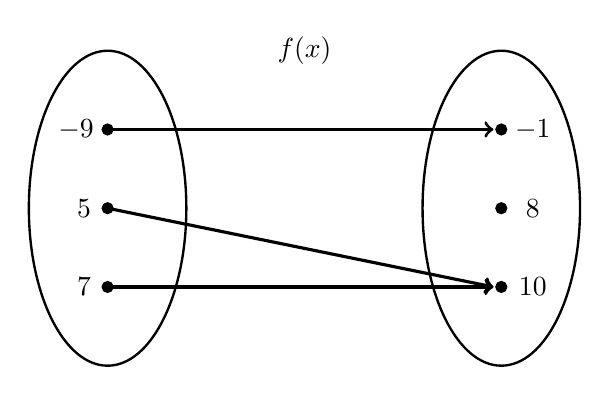
\begin{tikzpicture}
	\node at (2.5,2) {$f(x)$};
	% Ellipses
	\draw[line width=0.03cm] (0,0) circle (1 and 2);
	\draw[line width=0.03cm] (5,0) circle (1 and 2);
	
	% Nodes
	\draw[fill=black] (0,1) circle (0.07);
	\draw[fill=black] (0,0) circle (0.07);
	\draw[fill=black] (0,-1) circle (0.07);
	
	\draw[fill=black] (5,1) circle (0.07);
	\draw[fill=black] (5,0) circle (0.07);
	\draw[fill=black] (5,-1) circle (0.07);
	
	% Arrow
	\draw[line width=0.04cm,->] (0,1) -- (4.9,1);
	\draw[line width=0.04cm,->] (0,0) -- (4.9,-1);
	\draw[line width=0.04cm,->] (0,-1) -- (4.9,-1);
	
	% Labels
	\node at (-0.4,1) {$-9$};
	\node at (-0.3,0) {$5$};
	\node at (-0.3,-1) {$7$};
	
	\node at (5.4,1) {$-1$};
	\node at (5.4,0) {$8$};
	\node at (5.4,-1) {$10$};
	\end{tikzpicture}
	\]

\begin{enumerate}[(a)]
\item What is the domain of $f(x)$?
\item What is the codomain of $f(x)$?
\item What is the range of $f(x)$?
\end{enumerate} \pspace

\sol
{\itshape
\begin{enumerate}[(a)]
\item The domain of $f(x)$ is $\{ -9, 5, 7 \}$.

\item The codomain of $f(x)$ is $\{ -1, 8, 10 \}$.

\item The range of $f(x)$ is $\{ -1, 10 \}$. 
\end{enumerate}
}





\newpage





% Problem 5
\problem{10} Suppose $f(x)$ and $g(x)$ are the functions given below. 
        \begin{table}[!ht]
        \centering
        \begin{tabular}{| c || c | c | c | c | c | c | c |} \hline
	$x$ & $-2$ & $0$ & $1$ & $3$ & $4$ & $5$ & $10$ \\ \hline
	$f(x)$ & $-1$ & $-7$ & $5$ & $-2$ & $\pi$ & $19$ & $10$ \\ \hline
	$g(x)$ & $17$ & $1$ & $12$ & $0$ & $4$ & $8$ & $6$ \\ \hline
        \end{tabular}
        \end{table}

Compute the following: \pspace
        \begin{enumerate}[(a)]
        \item $f(1)= 5$ \vfill
        \item $g(0)= 1$ \vfill
        \item $(f + g)(5)= f(5) + g(5)= 19 + 8= 27$ \vfill
        \item $(f - g)(-2)= f(-2) - g(-2)= -1 - 17= -18$ \vfill
        \item $(6f)(1)= 6f(1)= 6(5)= 30$ \vfill
        \item $\left(\dfrac{f}{g}\right)(10)= \dfrac{f(10)}{g(10)}= \dfrac{10}{6}= \dfrac{5}{3}$ \vfill
        \item $f(4)\, g(5)= \pi \cdot 8= 8\pi$ \vfill
        \item $f(2 - g(0))= f(2 - 1)= f(1)= 5$ \vfill
        \item $(f \circ g)(0)= f(g(0))= f(1)= 5$ \vfill
        \item $(g \circ f)(3)= g(f(3))= g(-2)= 17$ \vfill
        \end{enumerate}





\newpage





% Problem 6
\problem{10} Suppose $f(x)$ and $g(x)$ are the functions given below. 
	\[
	\begin{aligned}
	f(x)&= 5x - 1 \\[0.3cm]
	g(x)&= x^2 + 2x + 3
	\end{aligned}
	\]

Compute the following: \pspace
\begin{enumerate}[(a)]
\item $f(1)= 5(1) - 1= 5 - 1= 4$ \vfill
\item $g(0)= 0^2 + 2(0) + 3= 0 + 0 + 3= 3$ \vfill
\item $f(1) - 2g(1)= \big( 5(1) - 1) \big) - 2 \big(1^2 + 2(1) + 3 \big)= 4 - 2(6)= 4 - 12= -8$ \vfill
\item $f(x) - g(x)= (5x - 1) - (x^2 + 2x + 3)= 5x - 1 - x^2 - 2x - 3= -x^2 + 3x - 4$ \vfill
\item $f(x) \, g(x)= (5x - 1)(x^2 + 2x + 3)= 5x^3 + 10x^2 + 15x - x^2 - 2x - 3= 5x^3 + 9x^2 + 13x - 3$ \vfill
\item $\left( \dfrac{f}{g} \right)(x)= \dfrac{5x - 1}{x^2 + 2x + 3}$ \vfill
\item $(g \circ f)(1)= g(f(1))= g(4)= (4)^2 + 2(4) + 3= 16 + 8 + 3= 27$ \vfill
\item $f(g(0))= f(3)= 5(3) - 1= 15 - 1= 14$ \vfill
\item $(f \circ g)(x)= f(g(x))= f(x^2 + 2x + 3)= 5(x^2 + 2x + 3) - 1= 5x^2 + 10x + 15 - 1= 5x^2 + 10x + 14$ \vfill
\item $(g \circ f)(x)= g(f(x))= g(5x - 1)= (5x - 1)^2 + 2(5x - 1) + 3= 25x^2 - 10x + 1 + 10x - 2 + 3= 25x^2 + 2$ \vfill
\end{enumerate}


%\printpoints
\end{document}